\documentclass{article}
\usepackage[T2A]{fontenc}
\usepackage[utf8]{inputenc}
\usepackage[russian]{babel}
\usepackage{graphicx}

\begin{document}

\title{Практика № 1}
\author{Ращупкин Е., Боков Е., Мишунин Н.}
\maketitle

\section{Задача 1}
Диск состоит из пронумерованных кластеров. На диске есть именованные папки, в которые вложены папки или именованные файлы. Список файлов и папок в папке хранится в одном кластер диска, данные файлов хранятся в нескольких кластерах.

\begin{itemize}
    \item Выделите классы и определите отношения между ними, используя абстрактные типы данных (АТД) и метод Аббота.
    \item Добавьте операции и атрибуты к имеющимся классам для создания, удаления папок и файлов, записи и чтения буфера данных с определенной позиции в файле.
\end{itemize}

\begin{verbatim}
@startuml
class Disk {
    - clusters: List<Cluster>
    - folders: List<Folder>
    + addFolder(folder: Folder): void
    + removeFolder(folder: Folder): void
    + addCluster(cluster: Cluster): void
    + removeCluster(cluster: Cluster): void
}

class Cluster {
    - id: int
    - folders: List<Folder>
    - files: List<File>
    + addFolder(folder: Folder): void
    + removeFolder(folder: Folder): void
    + addFile(file: File): void
    + removeFile(file: File): void
}

class Folder {
    - name: String
    - subFolders: List<Folder>
    - files: List<File>
    + addSubFolder(folder: Folder): void
    + removeSubFolder(folder: Folder): void
    + addFile(file: File): void
    + removeFile(file: File): void
}

class File {
    - name: String
    - data: Data
    + writeData(buffer: byte[], position: int): void
    + readData(buffer: byte[], position: int): byte[]
}

class Data {
    - clusters: List<Cluster>
    + addCluster(cluster: Cluster): void
    + removeCluster(cluster: Cluster): void
}

'Диск состоит из пронумерованных кластеров
Disk "1" *-- "1.." Cluster

'На диске есть именованные папки
Disk "1" o-- "0.." Folder

'именованные папки, в которые вложены папки
Folder "1" o-- "0.." Folder 

'Или именованные файлы
Folder "1" -- "0.." File

'Файл содержит данные
File "1" *-- "1" Data

'Данные файлов хранятся в нескольких кластерах
Data "1" -- "1.." Cluster

'Список папок в папке хранится в одном кластер диска
Folder "0.." o-- "1" Cluster

'Список папок в папке хранится в одном кластер диска
File "0.." o-- "1" Cluster
@enduml
\end{verbatim}

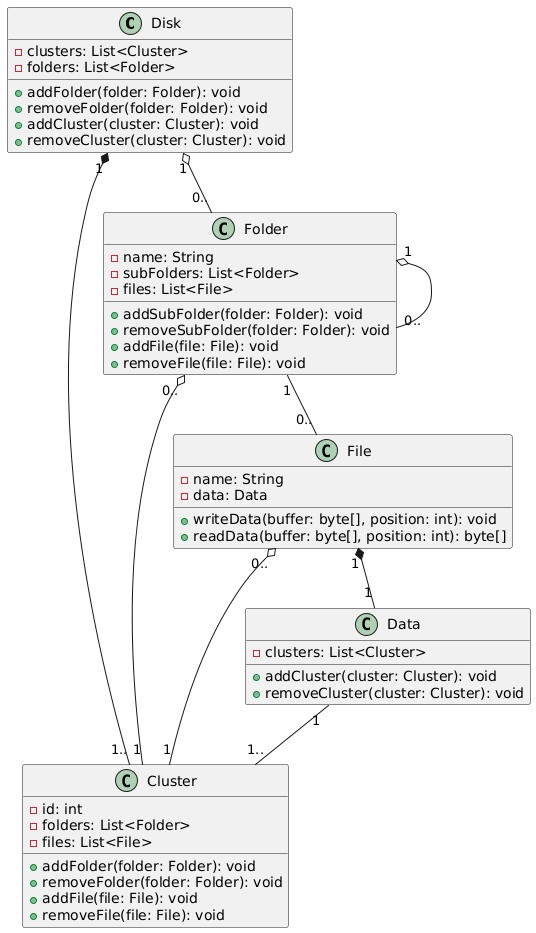
\includegraphics[width=\textwidth]{1.png}

\section{Задача 2}
Больной посещает доктора, чтобы получить рецепт на лекарства от своей болезни.

\begin{itemize}
    \item Выделите классы и постройте модель предметной области для системы учета посещений больными докторов для поликлиники.
    \item Выделите классы и постройте модель предметной области для программы-ежедневника для посетителей.
\end{itemize}

\section{Задача 3}
В межгосударственном стандарте по оценке качества программных средств ГОСТ 28195-89 качество характеризуется набором факторов. На каждом из этапов разработки программного средства фактор описывается набором критериев. Каждый критерий измеряется с помощью нескольких метрик, различающихся для этапов разработки.

\begin{itemize}
    \item Выделите классы и постройте структурную модель качества программных средств, используя метод именных групп.
    \item Используя схему, постройте критерии и метрики надежности для этапа реализации программного средства.
\end{itemize}

\begin{verbatim}
@startuml
class DevelopmentStage {
    +factors: Factor[]
    +DevelopmentStage(factors: Factor[]): DevelopmentStage
}

class Factor {
    +criterias: Criteria[]
    +Factor(criteria: Criteria[]): Factor
}

class Criteria {
    +metrics: Metric[]
    +Criteria(metrics: Metric[]): Criteria
}

class Metric {
    +estimatedProperties: EstimatedProperty[]
    +Metric(estimatedProperties: EstimatedProperty[]): Metric
}

class ReliabilityFactor {
    +criterias: FailoverCriteria[]
    +ReliabilityFactor(criterias: FailoverCriteria[]): ReliabilityFactor
}

class FailoverCriteria {
    +errorRateMetrics: ErrorRateMetric[]
    +recoveryTimeMetrics: RecoveryTimeMetric[]
    +ReliabilityFactor(errorRateMetrics: ErrorRateMetric[], recoveryTimeMetrics: RecoveryTimeMetric[]): ReliabilityFactor
}

class ErrorRateMetric {
    -numOfError: int32
    -timeWork: float
    +CalculateNumOfErrors(): int32
}

class RecoveryTimeMetric {
    -recoveryTime: double
    +CalculateRecoveryTime(): double
}

DevelopmentStage "1" *-- "*" Factor
Factor "1" *-- "*" Criteria
Criteria "1" *-- "*" Metric
ReliabilityFactor "1" *-- "*" FailoverCriteria
FailoverCriteria "1" *-- "*" ErrorRateMetric
FailoverCriteria "1" *-- "*" RecoveryTimeMetric
@enduml
\end{verbatim}

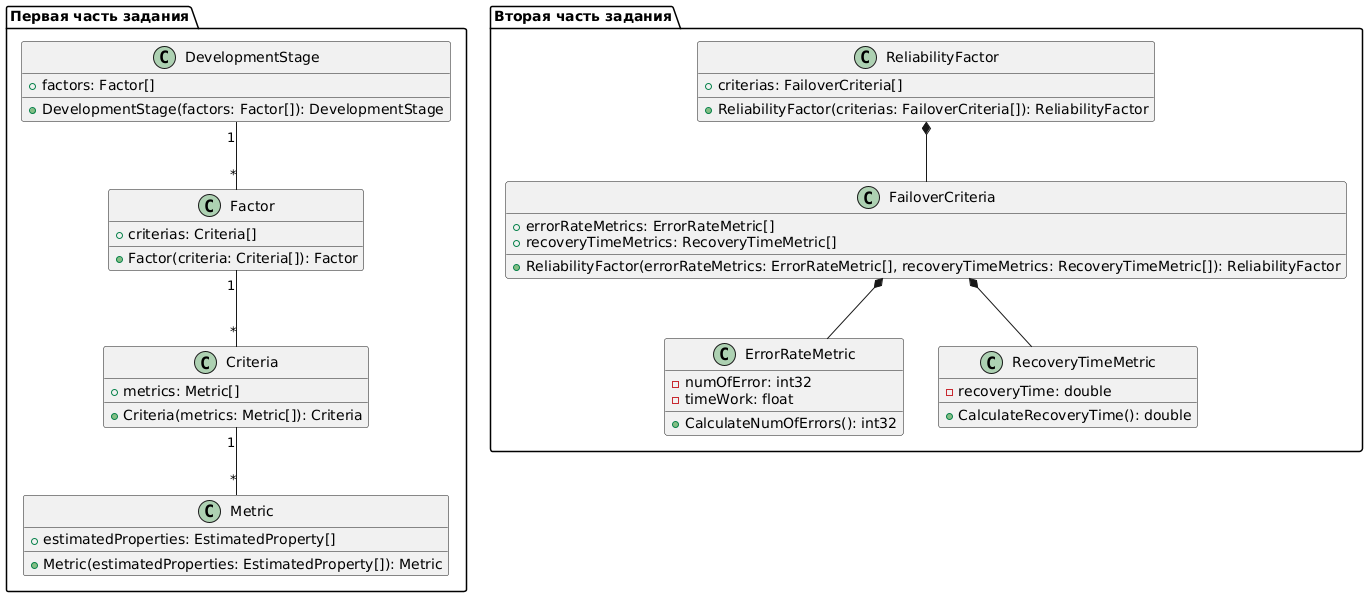
\includegraphics[width=\textwidth]{3.png}

\section{Задача 4}
Аудиоплееры состоят из менеджера плагинов, пользовательского интерфейса, который обрабатывает пользовательский ввод, управляющего компонента, реализующего основную функциональность, и мультимедиа-библиотеки.

\begin{itemize}
    \item Выделите классы и определите отношения между ними, используя АТД и метод Аббота.
    \item Для загрузки, включения и выключения плагинов добавьте операции и атрибуты к выделенным классам.
    \item Уточните описание управляющего компонента, чтобы в нем присутствовал менеджер сетевых подключений, и в системе в целом был сервер с базой доступных плагинов. Менеджер плагинов может, используя менеджер соединений, подключаться к серверу с целью проверки обновлений установленных плагинов.
    \item (*)Укажите, что результатом действий пользователя являются события в интерфейсе, и плагин может через менеджера зарегистрировать себя в качестве обработчика этих событий
\end{itemize}

\subsubsection{Рекомендации по выполнении задания 4}
Создать абстрактный класс Event и интерфейс Listener с операцией handleEvent с параметром типа Event, реализуемых Plugin и PluginManagerю Определить реализуемый PluginManager интерфейс Subject с общедоступным свойством listeners типа Listener кратности не меньше нуля. При возникновении события UI вызывает handleEvent в классе PluginManager и передает событие event. PluginManager вызывает handleEvent у каждого элемента listeners.

\begin{verbatim}
@startuml
abstract class Event {
    - String eventType
    + String getEventType()
}

interface Listener {
    + void handleEvent(Event event)
}

interface Subject {
    + void registerListener(Listener listener)
    + void notifyListeners(Event event)
}

class AudioPlayer {
    - PluginManager pluginManager
    - UserInterface ui
    - MediaLibrary mediaLibrary
    + void loadMedia()
    + void play()
    + void pause()
    + void stop()
}

class PluginManager implements Subject {
    - List<Plugin> plugins
    - ConnectionManager connectionManager
    - List<Listener> listeners
    + void loadPlugin(Plugin plugin)
    + void enablePlugin(Plugin plugin)
    + void disablePlugin(Plugin plugin)
    + void checkForUpdates()
    + void registerListener(Listener listener)
    + void notifyListeners(Event event)
}

class Plugin {
    - String name
    - String version
    + void handleEvent(Event event)
}

class UserInterface {
    - AudioPlayer audioPlayer
    + void getUserInput()
    + void display()
}

class MediaLibrary {
    - List<MediaFile> mediaFiles
    + void addMediaFile(MediaFile mediaFile)
    + void removeMediaFile(MediaFile mediaFile)
    + List<MediaFile> getMediaFiles()
}

class MediaFile {
    - String title
    - String filePath
    + String getTitle()
    + String getFilePath()
}

class ConnectionManager {
    - String serverUrl
    + void connect()
    + void disconnect()
    + void checkForUpdates()
}
'Аудиоплееры состоят из менеджера плагинов
AudioPlayer "1" *-- "1" PluginManager
'Аудиоплееры состоят из пользовательского интерфейса, который обрабатывает пользовательский ввод
AudioPlayer "1" *-- "1" UserInterface
'Аудиоплееры состоят из мультимедиа-библиотеки
AudioPlayer "1" *-- "1" MediaLibrary
'Уточните описание управляющего компонента, чтобы в нем присутствовал менеджер сетевых подключений
PluginManager "1" *-- "1" ConnectionManager
'Менеджер плагинов может, используя менеджер соединений, подключаться к серверу с целью проверки обновлений установленных плагинов
PluginManager "1" o-- "0..*" Plugin 
'Плагин может через менеджера зарегистрировать себя в качестве обработчика этих событий
Plugin "1" ..|> "0..1" Listener
'PluginManager реализует интерфейс Subject с общедоступным свойством listeners типа Listener
PluginManager "1" ..|> "0..*" Listener
@enduml
\end{verbatim}

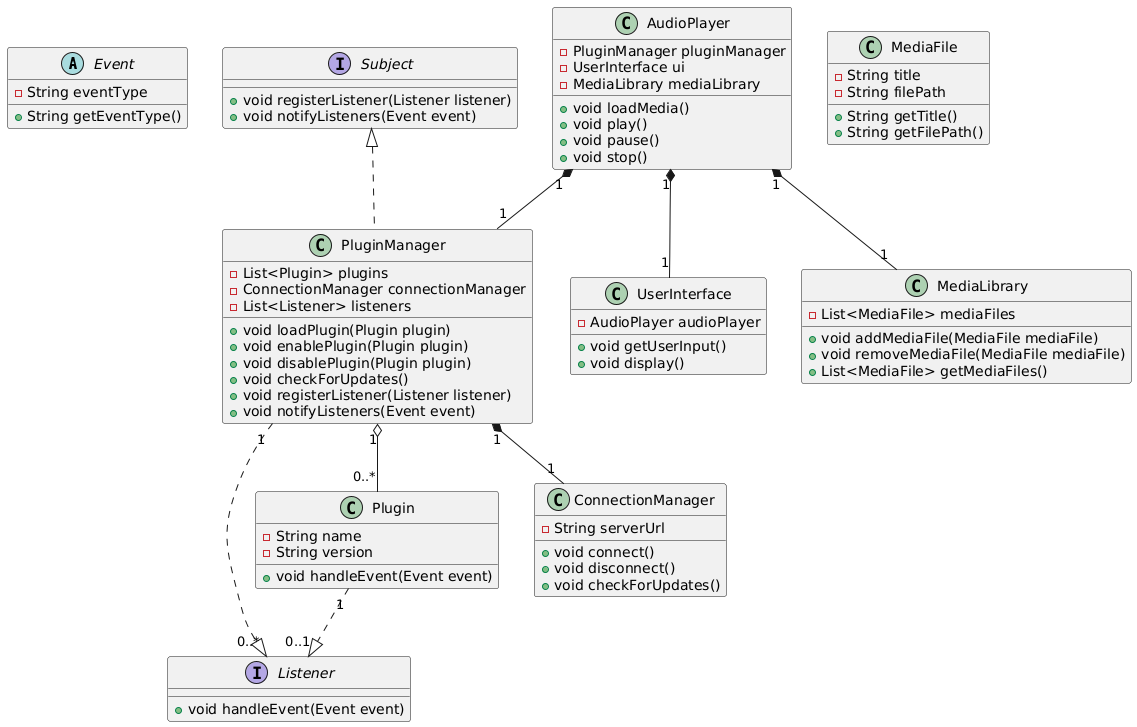
\includegraphics[width=\textwidth]{4.png}

\section{Задача 5}
Рассчитать оценку диаграммы классов, сделать вывод


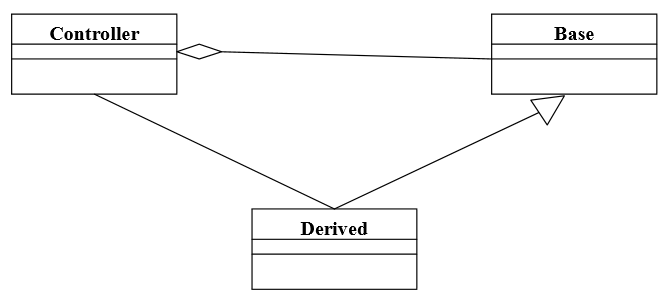
\includegraphics[width=\textwidth]{task5.png}

$ S = \frac{(5 + 5 + 5) + (1 + 3 + 2)}{1 + 3 + \sqrt{1 + 3}} = 3.5 $

\section{Задача 6}
Рассчитать оценку диаграммы классов, сделать вывод

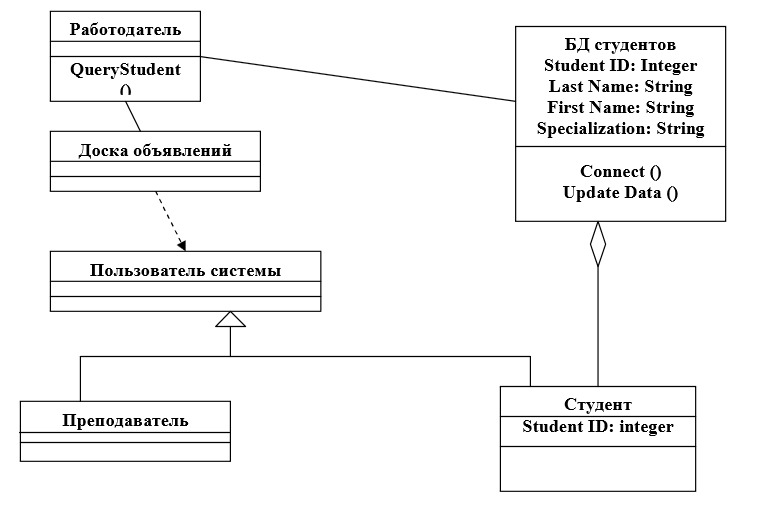
\includegraphics[width=\textwidth]{task6.png}

\section{Задача 7}
Рассчитать оценку диаграммы классов, сделать вывод

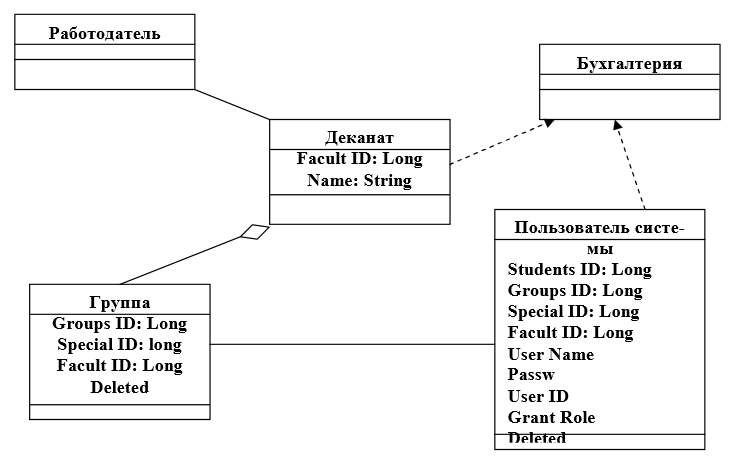
\includegraphics[width=\textwidth]{task7.png}

\end{document}
